\documentclass{article}

\usepackage{fancyhdr}
\usepackage{extramarks}
\usepackage{amsmath}
\usepackage{amsthm}
\usepackage{amsfonts}
\usepackage{tikz}
\usepackage[plain]{algorithm}
\usepackage{algpseudocode}
\usepackage{enumerate}
\usepackage{amssymb}
\usepackage{tikz}
\usetikzlibrary{automata,positioning,arrows}

\usetikzlibrary{automata,positioning}

%
% Basic Document Settings
%

\topmargin=-0.45in
\evensidemargin=0in
\oddsidemargin=0in
\textwidth=6.5in
\textheight=9.0in
\headsep=0.25in

\linespread{1.1}

\pagestyle{fancy}
\lhead{\hmwkAuthorName}
\chead{\hmwkClass:\ \hmwkTitle}
\rhead{\firstxmark}
\lfoot{\lastxmark}
\cfoot{\thepage}

\renewcommand\headrulewidth{0.4pt}
\renewcommand\footrulewidth{0.4pt}

\setlength\parindent{0pt}
\setlength{\parskip}{5pt}

%
% Create Problem Sections
%

\newcommand{\enterProblemHeader}[1]{
    \nobreak\extramarks{}{Problem \arabic{#1} continued on next page\ldots}\nobreak{}
    \nobreak\extramarks{Problem \arabic{#1} (continued)}{Problem \arabic{#1} continued on next page\ldots}\nobreak{}
}

\newcommand{\exitProblemHeader}[1]{
    \nobreak\extramarks{Problem \arabic{#1} (continued)}{Problem \arabic{#1} continued on next page\ldots}\nobreak{}
    \stepcounter{#1}
    \nobreak\extramarks{Problem \arabic{#1}}{}\nobreak{}
}

\setcounter{secnumdepth}{0}
\newcounter{partCounter}
\newcounter{homeworkProblemCounter}
\setcounter{homeworkProblemCounter}{1}
\nobreak\extramarks{Problem \arabic{homeworkProblemCounter}}{}\nobreak{}

%
% Homework Problem Environment
%
% This environment takes an optional argument. When given, it will adjust the
% problem counter. This is useful for when the problems given for your
% assignment aren't sequential. See the last 3 problems of this template for an
% example.
%
\newenvironment{homeworkProblem}[1][-1]{
    \ifnum#1>0
        \setcounter{homeworkProblemCounter}{#1}
    \fi
    \section{Problem \arabic{homeworkProblemCounter}}
    \setcounter{partCounter}{1}
    \enterProblemHeader{homeworkProblemCounter}
}{
    \exitProblemHeader{homeworkProblemCounter}
}

\newcommand\abs[1]{\lvert~#1~\rvert}
\newcommand{\st}{\mid}

\newcommand{\cmark}{\ding{51}}
\newcommand{\xmark}{\ding{55}}
 
\newcommand{\SUBSTRING}{\textsc{Substring}}
\newcommand{\REP}{\textsc{Rep}}
\newcommand{\blank}{\scalebox{1.5}{\textvisiblespace}}

%
% Homework Details
%   - Title
%   - Due date
%   - Class
%   - Section/Time
%   - Instructor
%   - Author
%

\newcommand{\hmwkTitle}{Homework\ \#1}
\newcommand{\hmwkDueDate}{Jan 19, 2023}
\newcommand{\hmwkClass}{CSE 105}
\newcommand{\hmwkClassInstructor}{Professor Minnes}
\newcommand{\hmwkAuthorName}{\textbf{Ray Tsai}}
\newcommand{\hmwkPID}{A16848188}

%
% Title Page
%

\title{
    \vspace{2in}
    \textmd{\textbf{\hmwkClass:\ \hmwkTitle}}\\
    \normalsize\vspace{0.1in}\small{Due\ on\ \hmwkDueDate\ at 23:59pm}\\
    \vspace{0.1in}\large{\textit{\hmwkClassInstructor}} \\
    \vspace{3in}
}

\author{
  \hmwkAuthorName \\
  \vspace{0.1in}\small\hmwkPID
}
\date{}

\renewcommand{\part}[1]{\textbf{\large Part \Alph{partCounter}}\stepcounter{partCounter}\\}

%
% Various Helper Commands
%

% Useful for algorithms
\newcommand{\alg}[1]{\textsc{\bfseries \footnotesize #1}}

% For derivatives
\newcommand{\deriv}[1]{\frac{\mathrm{d}}{\mathrm{d}x} (#1)}

% For partial derivatives
\newcommand{\pderiv}[2]{\frac{\partial}{\partial #1} (#2)}

% Integral dx
\newcommand{\dx}{\mathrm{d}x}

% Probability commands: Expectation, Variance, Covariance, Bias
\newcommand{\Var}{\mathrm{Var}}
\newcommand{\Cov}{\mathrm{Cov}}
\newcommand{\Bias}{\mathrm{Bias}}
\newcommand*{\Z}{\mathbb{Z}}
\newcommand*{\Q}{\mathbb{Q}}
\newcommand*{\R}{\mathbb{R}}
\newcommand*{\C}{\mathbb{C}}
\newcommand*{\N}{\mathbb{N}}
\newcommand*{\prob}{\mathds{P}}
\newcommand*{\E}{\mathds{E}}

\begin{document}

\maketitle

\pagebreak

\begin{homeworkProblem}
  With $\Sigma_1 = \{0,1\}$ and $\Sigma_2 = \{a,b,c,d,e,f,g,h,i,j,k,l,m,n,o,p,q,r,s,t,u,v,w,x,y,z\}$
  and $\Gamma = \{0,1,x,y,z\}$

  \begin{enumerate}[(a)]
    \item Give an example of the shortest string over $\Sigma_1$ that is meaningful to you in some
    way, and explain why it's meaningful to you.

    \begin{proof}[Solution]
      The empty string $\epsilon_1 \in \Sigma_1^*$ is meaningful to me  because it's the shortest
      string.
    \end{proof}

    \item List all examples of strings of length $1$ over $\Sigma_2$ and explain why your list is
    exhaustive.

    \begin{proof}[Solution]
      Since a string of length $1$ is simply a string of a single symbol, each symbol and only the
      symbol in $\Sigma_2$ are strings of length 1, namely
      \[
        a,b,c,d,e,f,g,h,i,j,k,l,m,n,o,p,q,r,s,t,u,v,w,x,y,z.
      \]
    \end{proof}

    \item Calculate the number of distinct strings of length 3 over $\Gamma$ and explain your
    calculation.

    \begin{proof}[Solution]
      Since there are $5$ choices for each character there are $3$ characters in the string, there
      are $5^3 = 125$ distinct strings of length 3 over $\Gamma$.
    \end{proof}

    \item With the ordering $x < y < z < 0 < 1$, list the first ten strings over $\Gamma$ in string
    order.

    \begin{proof}[Solution]
      $\epsilon, x, y, z, 0 , 1, xx, xy, xz, x0$
    \end{proof}

    \item Give an example of a finite set that is a language over $\Sigma_1$ and over $\Sigma_2$ and
    over $\Gamma$, or explain why there is no such set.

    \begin{proof}[Solution]
      Since $\Sigma_1^* \cup \Sigma_2^* \cup \Gamma^* = \{\epsilon\}$, $\{\epsilon\}$ is a language
      over all three alphabets.
    \end{proof}
    
    \item  Give an example of an infinite set that is a language over $\Sigma_1$  and over $\Gamma$,
    or explain why there is no such set.

    \begin{proof}[Solution]
      $(\Sigma_1 \cap \Gamma)^*$ is a language over $\Sigma_1$ and over $\Gamma$. Since $\Sigma_1
      \cap \Gamma$ is nonempty, $(\Sigma_1 \cap \Gamma)^*$ is an infinite set.
    \end{proof}
    \end{enumerate}
\end{homeworkProblem}

\newpage

\begin{homeworkProblem}
  \begin{enumerate}[(a)]
    \item Give three regular expressions that all describe the set of all strings over $\{a,b\}$
    that have even length. Ungraded bonus challenge: Make the expressions as different as possible!

    \begin{proof}[Solution]
      $((a \cup b)(a \cup b))^*, ((aa) \cup (ab) \cup (ba) \cup (bb))^*, (aa)^* \cup (ab)^* \cup
      (ba)^* \cup (bb)^*$.
    \end{proof}

    \item A friend tells you that each regular expression that has a Kleene star ($~^*$) describes
    an infinite language. Are they right? Either help them justify their claim or give a
    counterexample to disprove it and then fix the formula.

    \begin{proof}
      Yes they are correct. Suppose for the sake of contradiction that $\Sigma^*$ is finite, for a
      nonempty set $\Sigma$. Let $\sigma$ be concatenation of all strings in $\Sigma^*$. Consider
      $\sigma a$, for some $a \in \Sigma$. $\sigma a$ is a string over $\Sigma$, so $\sigma a \in
      \Sigma^*$. However, $\sigma a$ does not equal to any string in $\Sigma^*$, contradiction.
      Therefore, $\Sigma^*$ must be infinite.
    \end{proof}
  \end{enumerate}
\end{homeworkProblem}

\newpage

\begin{homeworkProblem}
  For languages $L_1, L_2$ over the alphabet $\Sigma_1 = \{0,1\}$, we have the associated sets of
  strings
  \[
    SUBSTRING(L_1) = \{ w \in \Sigma_1^* ~|~ \text{there exist } a,b \in \Sigma_1^* \text{ such that } awb \in L_1\}
  \]
  and 
  \[
    L_1 \circ L_2 = \{ w \in \Sigma_1^* ~|~ w = uv \text{ for some strings } u \in L_1 \text{ and } v \in L_2 \}
  \]
  \begin{enumerate}[(a)]
  \item Specify an example language $A$ over $\Sigma_1$ such that $A \neq \emptyset$ and yet
  $\SUBSTRING(A) = \emptyset$, or explain why there is no such example. A complete solution will
  include either (1) a precise and clear description of your example language $A$ and a precise and
  clear description of the result of computing $\SUBSTRING(A)$ using relevant definitions to justify
  this description and to justify the set equality with $\emptyset$, or (2) a sufficiently general
  and correct argument why there is no such example, referring back to the relevant definitions.

  \begin{proof}[Solution]
    There are no such examples. Since $A \neq \emptyset$, let $w \in A$. There exists $a =
    \epsilon$, $b = \epsilon$ in $\Sigma_1^*$ such that $awb = w \in A$, so $w \in \SUBSTRING(A)$.
    Thus, $\SUBSTRING(A)$ must be nonempty.
  \end{proof}

  \item Specify example languages $B, C$ over $\Sigma_1$ such that $B \neq \Sigma_1^*$ and $C \neq
  \Sigma_1^*$ and yet $B \circ C = \Sigma_1^*$, or explain why there are no such examples. A
  complete solution will include either (1) a precise and clear description of your example
  languages $B,C$ and a precise and clear description of the result of computing $B \circ C$ using
  relevant definitions to justify this description and to justify the set equality with
  $\Sigma_1^*$, or (2) a sufficiently general and correct argument why there is no such example,
  referring back to the relevant definitions.

  \begin{proof}[Solution]
    Consider $B = \{w \in \Sigma_1^* \, | \, |w| \text{ is even}\}$ and $C = \{w \in \Sigma_1^* \, |
    \, |w| \text{ is odd}\} \cup \{\epsilon\}$. Let $b \in B$ and $c \in C$. When $c \neq \epsilon$,
    we know $bc$ is of odd length. Otherwise, $bc = b$ is of even length. Hence, we get $$B \circ C
    = \{w \in \Sigma_1^* \, | \, |w| \text{ is even}\} \cup \{w \in \Sigma_1^* \, | \, |w| \text{ is
    odd}\} = \Sigma_1^*.$$
  \end{proof}

  \item Specify example {\bf finite} languages $L_1, L_2$ over $\Sigma_1$ such that $L_1 \circ L_2
  \neq L_1$ but $|L_1 \circ L_2| = |L_1|$, or explain why there are no such examples. A complete
  solution will include either (1) a precise and clear description of your example languages $L_1,
  L_2$ and a precise and clear description of the result of computing $L_1 \circ L_2$ using relevant
  definitions to justify this description and to justify the cardinality claims and set (in)equality
  claims, or (2) a sufficiently general and correct argument why there is no such example, referring
  back to the relevant definitions.

  \begin{proof}[Solution]
    Consider $L_1 = \{\epsilon\}$ and $L_2 = \{1\}$. $L_1 \circ L_2 = \{1\} \neq L_1$, but $\abs{L_1
    \circ L_2} = \abs{\{1\}} = \abs{L_1}$.
  \end{proof}
  \end{enumerate}
\end{homeworkProblem}

\newpage

\begin{homeworkProblem}
  Consider the finite automaton $(Q, \Sigma, \delta, q_0, F)$ whose state diagram is depicted below
  \begin{center}
  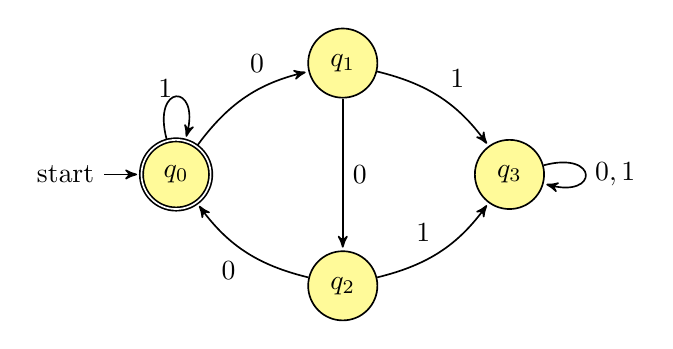
\begin{tikzpicture}[->,>=stealth',shorten >=1pt, auto, node distance=2cm, semithick]
  \tikzstyle{every state}=[text=black, fill=yellow!40]

  \node[initial,state, accepting] (q0)          {$q_0$};
  \node[state]         (q1) [above right of=q0, xshift=20pt] {$q_1$};
  \node[state]         (q2) [below right of=q0, xshift=20pt] {$q_2$};
  \node[state]         (q3) [below right of=q1, xshift=20pt] {$q_3$};

  \path (q0) edge  [loop above, near start] node {$1$} (q0)
          edge [bend left=20, near end] node {$0$} (q1)
      (q1) edge [bend left=0] node {$0$} (q2)
          edge [bend left=20] node {$1$} (q3)
      (q2) edge [bend left=20] node {$0$} (q0)
          edge [bend right=20] node {$1$} (q3)
      (q3) edge [loop right] node {$0,1$} (q3)
  ;
  \end{tikzpicture}
  \end{center}
  where $Q = \{q_0, q_1, q_2, q_3\}$, $\Sigma = \{0,1\}$, and $F = \{q_0\}$, and $\delta: Q \times
  \Sigma \to Q$ is specified by the look-up table
  \begin{center}
  \begin{tabular}{c|cc}
          & $0$ & $1$ \\
      \hline
    $q_0$ & $q_1$ & $q_0$ \\
    $q_1$ & $q_2$ & $q_3$ \\
    $q_2$ & $q_0$ & $q_3$ \\
    $q_3$ & $q_3$ & $q_3$
  \end{tabular}
  \end{center}
  \begin{enumerate}[(a)]
    \item  A friend tries to summarize the transition function with the formula
    \[
      \delta(q_i,x) = \begin{cases}
        q_0 &\text{ when $i=0$ and $x=1$} \\
        q_3 &\text{ when $0<i\leq 3$ and $x=1$}\\
        q_j &\text{ when $j = (i+1) \mod 3$ and $x=0$}
      \end{cases}
    \]
    Are they right? Either help them justify their claim or give a counterexample to disprove it.

    \begin{proof}[Solution]
      The output $\delta(q_3, 0) = q_1$ is incorrect. It should be $q_3$ instead.
    \end{proof}

    \item Give a regular expression $R$ so that $L(R)$ is the language recognized by this finite
    automaton. Justify your answer by referring to the definition of the semantics of regular
    expressions and computations of finite automata. Include an explanation for why each string in
    $L(R)$ is accepted by the finite automaton {\it and} for why each string not in $L(R)$ is
    rejected by the finite automaton.

    \begin{proof}[Solution]
      Consider $R = (1 \cup 000)^*$. Suppose $w \in L(R)$. We may assume $w \neq \epsilon$, as the
      start state is the end state so $\epsilon$ would be accepted. Then, $w$ consists of sequences
      of $1$ and $000$. Denote $\delta(\delta(\delta(q_0, 0), 0), 0)$ as $\delta(q_0, 000)$. At the
      start state, if the automaton reads $000$, we get $\delta(q_0, 000) = q_0$, so we end up at
      the start state. Otherwise, the automaton reads $1$ and $\delta(q_0, 1) = q_0$. Thus, $w$ is
      guaranteed to end up at the start state, which is also the end state, so any string $w \in
      L(R)$ would be accepted. 
      
      Now suppose that $w \notin L(R)$. Since the prefix of the form $1$ or $000$ takes no effect,
      we may removed them from $w$. If $w = 0$ or $w = 00$, then $\delta(q_0, 0) = q_1$ and
      $\delta(\delta(q_0, 0), 0) = q_2$, which would get rejected because it doesn't end in the
      accept state. Thus, we may assume $w$ starts with $01$ or $001$. Then, $\delta(\delta(q_0, 0),
      1) = \delta(\delta(\delta(q_0, 0), 0), 1) = q_3$. However, note that $\delta(q_3, x) = q_3$
      for all $x \in \Sigma$, so the automaton would get stuck in $q_3$ once it is reached, which
      implies that $w$ would never end up in the accept state. Thus, $w$ would get rejected by the
      automaton.
    \end{proof}

    \newpage

    \item  Keeping the same set of states $Q = \{q_0, q_1, q_2, q_3\}$, alphabet $\Sigma = \{0,1\}$,
    same start state $q_0$, and same transition function $\delta$, choose a new set of accepting
    states $F_{new}$ so that the new finite automaton that results accepts at least one string that
    the original one rejected {\bf and} rejects at least one string that the original one accepted,
    or explain why there is no such choice of $F_{new}$. A complete solution will include either (1)
    a precise and clear description of your choice of $F_{new}$ and a precise and clear the two
    example strings using relevant definitions to justify them, or (2) a sufficiently general and
    correct argument why there is no such example, referring back to the relevant definitions.

    \begin{proof}[Solution]
      Consider $F_{new} = \{q_3\}$. Since $01$ ends in $q_3$, it is accepted by the new automaton
      but not by the original one. Since all strings that the original automaton accepts end in
      $q_0$, they would all be rejected by the new automaton.
    \end{proof}
  \end{enumerate}
\end{homeworkProblem}
\end{document}